\chapter{Target Cipher Specifications \& Architectures}
\label{ch:ciphers}

\section{The BAKSHEESH Block Cipher}
\label{sec:baksheesh_spec}
BAKSHEESH~\cite{baksi2023baksheesh} is an iterative lightweight Substitution-Permutation Network (SPN) operating on a 128-bit block with a 128-bit master key. It executes \textbf{35 identical rounds}, followed by a post-whitening key addition. The 128-bit state $X$ is partitioned into 32 four-bit nibbles:
\begin{equation}
    X = (w_{31} \parallel w_{30} \parallel \dots \parallel w_1 \parallel w_0), \quad w_i \in \mathbb{F}_2^4
\end{equation}

\subsection{Round Function Pipeline}
Each round $r \in \{1, 2, \dots, 35\}$ applies four consecutive transformations:
\begin{enumerate}
    \item \textbf{SubCells}: Applies the identical 4-bit S-Box $S$ independently to all 32 nibbles:
    \begin{equation}
        w_i \leftarrow S[w_i], \quad 0 \le i \le 31
    \end{equation}
    \item \textbf{PermBits}: Applies the GIFT-128 bit permutation $P_{128}$ to the 128 bits of the state:
    \begin{equation}
        b_{P_{128}(k)} \leftarrow b_k, \quad 0 \le k \le 127
    \end{equation}
    where $P_{128}(k) = 4 \lfloor k / 16 \rfloor + 32 ((k \pmod{16}) \pmod 4) + \lfloor (k \pmod{16}) / 4 \rfloor$.
    \item \textbf{AddConstants}: A 6-bit round constant generated by an affine LFSR is XORed into specified state tap positions $\{8, 13, 19, 35, 67, 106\}$.
    \item \textbf{AddRoundKey}: The full 128-bit round subkey $K_r$ is XORed across the entire state:
    \begin{equation}
        X \leftarrow X \oplus K_r
    \end{equation}
\end{enumerate}

\begin{figure}[!htbp]
\centering
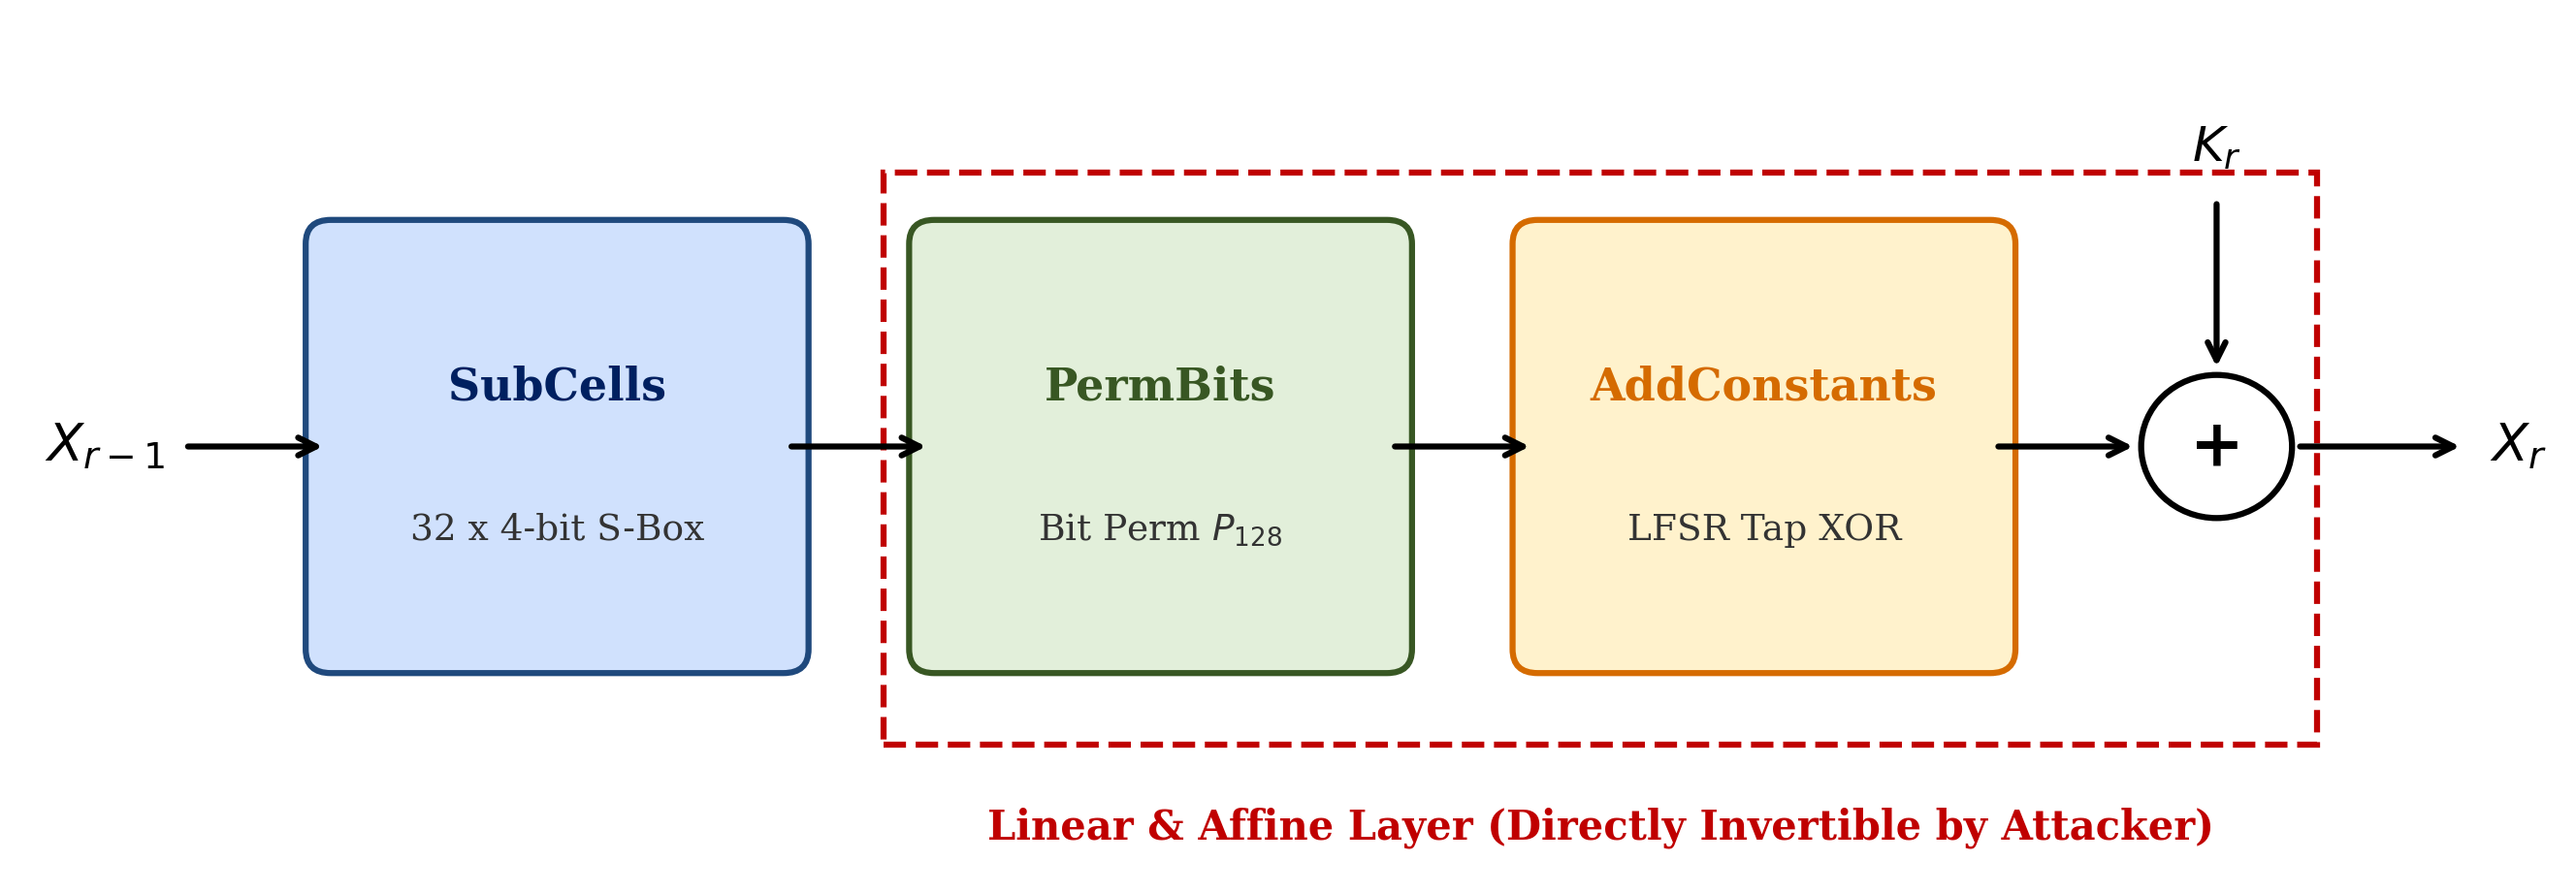
\includegraphics[width=0.88\linewidth]{figures/fig1_baksheesh_round.png}
\caption{One round of BAKSHEESH. \texttt{PermBits}, \texttt{AddConstants}, and \texttt{AddRoundKey} form a linear and affine layer that is directly invertible by an attacker.}
\label{fig:baksheesh_round}
\end{figure}

\subsection{The 4-bit S-Box with Linear Structures}
The 4-bit S-box of BAKSHEESH is defined by the mapping:
\begin{equation}
    S = [3, 0, 6, 13, 11, 5, 8, 14, 12, 15, 9, 2, 4, 10, 7, 1]
\end{equation}
The S-box is an involution-derived bijection with differential uniformity 4 and non-linearity 4. Crucially, the S-box exhibits a \textbf{non-trivial linear structure}:
\begin{equation}
    S(x) \oplus S(x \oplus 0\text{xA}) = 0\text{xA}
\end{equation}
While this property reduces hardware gate count under Boolean masking, it provides zero inherent resistance against differential or linked fault attacks.

\subsection{128-bit Rotational Key Schedule}
BAKSHEESH uses an ultra-simple rotational key schedule:
\begin{equation}
    K_r = K \lll (r - 1)
\end{equation}
Every round subkey bit is an exact, direct, bijective rotation of the original master key $K$. Consequently, recovering the equivalent subkey in Round 35 directly yields the master key via a single inverse rotation.

\section{The GIFT-128 Block Cipher}
\label{sec:gift_spec}
GIFT-128~\cite{banik2017gift} is an established lightweight block cipher operating on a 128-bit block with a 128-bit key over \textbf{40 rounds}. It shares the same bit permutation $P_{128}$ as BAKSHEESH but differs fundamentally in its key injection and S-box.

\subsection{64-bit Narrow Key Injection}
In GIFT-128, \texttt{AddRoundKey} extracts only \textbf{64 key bits} per round from the 128-bit key state (words $U$ and $V$). These 64 bits are injected exclusively into bit positions $b_2$ and $b_1$ of each 4-bit nibble. \textbf{Bit positions $b_0$ and $b_3$ receive zero key injection in that round}.

\section{Structural Comparison: BAKSHEESH vs. GIFT-128}
\label{sec:cipher_comparison}
Table~\ref{tab:cipher_comparison} compares the structural parameters and fault-attack implications between both ciphers.

\begin{table}[!htbp]
\centering
\caption{Architectural Comparison: BAKSHEESH vs. GIFT-128.}
\label{tab:cipher_comparison}
\begin{tabular}{lccp{5.5cm}}
\toprule
\textbf{Architectural Parameter} & \textbf{BAKSHEESH} & \textbf{GIFT-128} & \textbf{Fault Security Implication} \\
\midrule
Total Rounds & 35 & 40 & GIFT provides 5 extra diffusion rounds \\
Algebraic Degree of S-Box & 2 & 3 & Degree 2 enables 3-share TI masking \\
Key Injection Width & \textbf{128 bits / round} & \textbf{64 bits / round} & \textbf{BAKSHEESH leaks master key in 1 round; GIFT requires 2-round peeling} \\
Key Schedule & 1-bit cyclic rotation & LFSR + word rotation & BAKSHEESH is directly invertible \\
Masking Shares (TI) & 3 shares & 4 shares & BAKSHEESH has $2.43\times$ smaller area \\
Rounds Attacked for LFA & \textbf{Round 35 (1 round)} & \textbf{Rounds 39 \& 40 (2 rounds)} & GIFT doubles the attack rounds \\
Candidate Keys Left & 16 candidates ($2^4$) & 256 candidates ($2^8$) & GIFT requires $16\times$ larger search space \\
\bottomrule
\end{tabular}
\end{table}
